
In our investigation of the existing BDD Testing Setup in \ac{RCE}, we have organized the examination into several distinct subsections. The initial~\cref{subsec:BuildingRCE} will focus on the practical steps associated with compiling \ac{RCE}, highlighting the procedures and challenges encountered during the successful compilation process. Subsequently, in~\cref{subsec:PreparingRCETests}, we will elaborate on the configuration requirements for \ac{RCE} to enable the execution of the built-in test suite. Furthermore,~\cref{subsec:BuiltinBDDTest} will center on our examination of the BDD Testing Setup, the tests themselves, and our findings after applying a black-box testing paradigm, exploring the fault tolerance of the built-in tests.

Finally, transitioning to~\cref{subsec:CodeReview}, we will undertake a more comprehensive code review of the actual source code. This thorough analysis involves examining how Cucumber is integrated within the codebase. We will unravel the complexities of the Gherkin $.feature$ files and their interconnection with the corresponding Step Definition Code. This in-depth exploration is designed to illuminate the construction and execution of testing scenarios within \ac{RCE}'s application.

\subsection{Compiling \ac{RCE} from Scratch}
\label{subsec:BuildingRCE}
Initiating the compilation of \ac{RCE} entails a multistep process. This procedure includes downloading Eclipse IDE for RCP and RAP Developers and modifying its \textit{ini} file to augment the Java heap size—a crucial adjustment aimed at alleviating potential memory overflow issues throughout the compilation process~\cite{rceDevGuide10x}.

Subsequently, the source-code must be obtained and imported into Eclipse. Multiple sources are available for obtaining the source code of \ac{RCE}, including the official RCE website. However, we opted to utilize the GitHub repository (\href{https://github.com/rcenvironment/rce-main}{RCE-Main GitHub Repository}) for several advantages. Choosing the GitHub repository allows us to access the code as a git repository rather than plain files, providing enhanced version control and collaboration capabilities. This decision aligns with modern development practices and facilitates a more seamless integration of the code into our development environment. Before importing the project into Eclipse, the guide states that the generation OSGI bindings must be enabled first. The generation of \textit{OSGI-INF} can be enabled by navigating to the Eclipse preferences (\textit{Window → Preferences}), accessing the \textit{Plugin Development → DS Annotations} page, and enabling the option to \textit{Generate descriptors for annotated sources}. Additionally, the output directory must be set to \textit{OSGI-INF/generated}~\cite{rceDevGuide10x}.

Once these steps are completed, the source code can be imported into Eclipse by adding it as an existing project. Following the import, the target platform, a critical step for supplying external artifacts such as the Eclipse RCP framework and various libraries, must be set\footnote{Note: There is currently a discrepancy between the repository location specified in the target files of the RCE GitHub repositories (\href{https://github.com/rcenvironment/rce/blob/master/de.rcenvironment/eclipse/tp/remote/default_release_or_snapshot.target}{rce} and \href{https://github.com/rcenvironment/rce-main/blob/main/de.rcenvironment/eclipse/tp/remote/default_release_or_snapshot.target}{rce-main}
) and the repository location referenced in the developer guide.}. For convenience, the guide recommends using the default target platform named \textit{default\_release\_or\_snapshot.target}, located under \textit{de.rcenvironment/eclipse/tp/remote} within the code base, by default~\cite{rceDevGuide10x}.

It is important to note that the full steps for applying the target platform are detailed in the developer guide. Following these procedures, successful compilation of \ac{RCE} was achieved. However, during the process on Linux, we encountered a specific issue, which, fortunately, was already documented in the developer guide. This issue required us to disable Windows-specific subprojects in the workspace for seamless compilation~\cite{rceDevGuide10x}. It is crucial to mention that using Eclipse IDE for RCP and RAP Developers is essential, as attempting to compile it on a regular Eclipse IDE for Java and DSL Developers proved unsuccessful. However, we can confirm that the latest Eclipse RCP Version 2023-12 also yielded positive compilation outcomes.

\subsection{Preparing and executing \ac{RCE}'s BDD Tests}
\label{subsec:PreparingRCETests}
In the process of compiling and launching \ac{RCE} successfully, we then proceeded to execute the built-in BDD tests. Contrary to expectations, these tests are not executed separately through Eclipse or similar platforms; instead, they are integrated into the \ac{RCE} application itself as console commands, and are included in every build by default. This decision may initially seem confounding, as this functionality is typically not of interest to regular users, but is more geared towards developers or system administrators. Furthermore, the incorporation of such functionality results in an expansion of the overall size of the \ac{RCE} bundle, even when it is not essential. We assume that this decision is based on the capability of \ac{RCE} to test multiple \ac{RCE} versions and builds through the built-in BDD tests, irrespective of the version being executed.

A full documentation of the command(s) for executing the tests can be found in the \ac{RCE} Developer Guide. For our tests the command, listed in~\cref{lst:run-tests-command}, was sufficient. The command requires two arguments. Firstly, the tests to be executed, and secondly, the version of \ac{RCE} on which the tests should be performed. For example, the example command \textit{run-test :all releases/10.5.0} results in the execution of the entire test suite, indicated by \textit{:all}, on the \ac{RCE} release version \textit{10.5.0}.

\begin{listing}[ht]
\caption{run-test command signature}
\label{lst:run-tests-command}
\begin{minted}{shell}
run-test[s] [--format pretty|json] 
    <comma-separated list of test ids> |--all
    <build id>
\end{minted}
\end{listing}


During the initial execution of the command, it becomes evident that a freshly bootstrapped \ac{RCE} instance is unable to execute the test suite; instead, it prompts an error message. This issue is associated with the necessary configuration of the \ac{IM} as a prerequisite for the test suite. Consequently, the \ac{IM} must be configured through \ac{RCE}'s configuration file. There, the \textit{instanceManagement} configuration block must be added. This block defines the root directory where work files and managed RCE test installations will be stored. An illustrative example configuration is provided in~\cref{lst:configuration-json}.

\begin{listing}
\caption{InstanceManagement block entry in \ac{RCE}'s configuration.json}
\label{lst:configuration-json}
\inputminted{json}{files/code/configuration.json}
\end{listing}

Upon adjusting the \ac{IM} config block and then reissuing the test command, the tests are executed as intended. Throughout this process, crucial information, such as the test status and potential errors, is presented in the console. This output is depicted in~\cref{fig:rce-test-output}. The result is the successful completion of all tests without errors, suggesting, at least on the surface, the accurate processing of tests by the application.

\begin{figure}
    \centering
    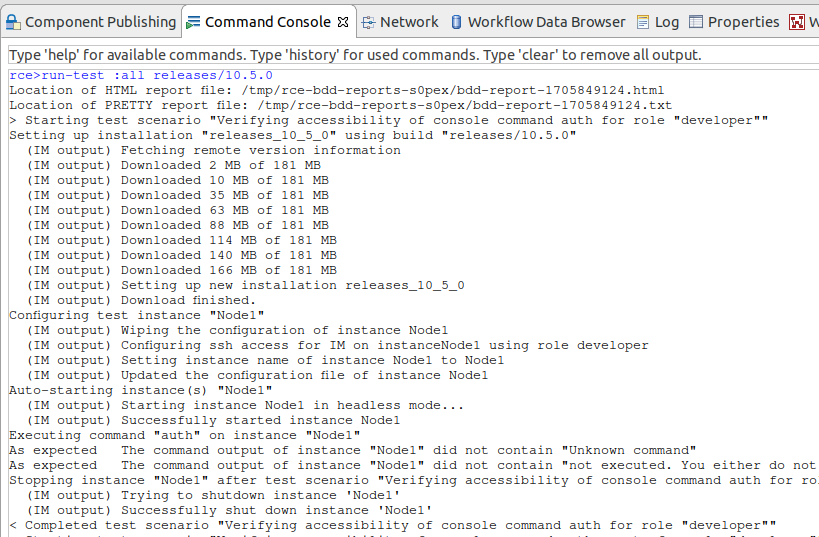
\includegraphics[width=\linewidth]{files/figures/rce-execute-tests.png}
    \caption{Example console output for command: "run-test :all releases/10.5.0"}
    \label{fig:rce-test-output}
\end{figure}


Although, in this step, we conducted only a very superficial black-box test through the execution of the tests, we were able to observed two noteworthy aspects. Firstly, the \ac{RCE} tests encompass a diverse range of test cases, covering both functional tests (component, network communication, remote-access, etc.) and \ac{GUI} functionalities. Exclusively in \ac{GUI} tests, \ac{RCE} is launched with an authentic \ac{GUI}, and the functionalities are explicitly emulated through simulated "virtual" clicks within the \ac{GUI}.
Executing the non-\acs{GUI}-based tests serves as a valuable test case, demonstrating that the typically \acs{GUI}-based application can successfully operate without a \acs{GUI}. This tests that the application can run on a server in a real-world scenario, i.e, without a display server. Additionally, it opens the possibility of integrating these tests into a CI/CD pipeline, which often lacks the aforementioned display server.

Secondly, it became apparent that the \ac{TSR} relies on the \ac{IM} to start multiple \ac{RCE} instances configured as either servers or clients.
Thus, proposing that the required logic for simulating a “distributed” environment heavily relies on the implementation of the \ac{IM} suggesting that it must be further analyzed in a subsequent step.

\subsection{\ac{RCE}'s BDD Testing Setup}
\label{subsec:BuiltinBDDTest}
In this subsection, we illuminate the workings of test execution. Initially, we provide a detailed overview of the setup and execution flow. Following that, we delve into how \ac{RCE} establishes a distributed system comprising multiple \ac{RCE} clients and servers locally. Next, we explain how \ac{RCE} overcomes the challenge of triggering behaviors and obtaining the state to properly evaluate the test cases across multiple clients and servers correctly. Lastly, we offer a brief summary and conclusion.

\subsubsection{\ac{RCE}'s Test Setup and Execution Details in RCE}
The specifics of the Test Setup are detailed in \ac{RCE}'s Developer Guide~\cite{rceDevGuide10x} and thoroughly discussed in the work by Mischke et al. (2022)~\cite{10.1007/978-3-031-08760-8_44}. In essence, the testing setup for \ac{RCE} revolves around the implementation of its test suite through a specialized component, referred to as \acf{TSR}. This component assumes the responsibility of interpreting Gherkin files and executing tests under predefined conditions. To process Gherkin files, the \ac{TSR} leverages the Cucumber library~\cite{10.1007/978-3-031-08760-8_44}, facilitating the mapping of free expressions in Gherkin to corresponding actions executed during the tests.

Within the Gherkin feature files, the "GIVEN" clauses stipulate, for example, that \ac{TSR} must initiate multiple client and server instances of \ac{RCE}. This initiation is facilitated by delegating the launch of numerous \ac{RCE} instances via the \acf{IM}~\cite{rceDevGuide10x}. 
The \ac{IM} plays a crucial role in overseeing \ac{RCE} instances used for testing purposes, which includes tasks such as downloading \ac{RCE}, initiating, and terminating instances~\cite{10.1007/978-3-031-08760-8_44,rceDevGuide10x}. Given that the tests can be initiated even in a localized environment without a network connection, emphasizing the self-sufficiency of the testing process and providing flexibility in conducting tests in isolated settings without external dependencies, the need for \ac{IM} to initiate the required instances locally becomes apparent.

This assumption can be easily verified using tools such as the Task Manager, Process Hacker, htop, etc. Upon scrutiny of Process Hacker during the tests, it becomes apparent that individual \ac{RCE} instances are initiated as subprocesses from the primary \ac{RCE} instance. This observation aligns with the test description provided by Mischke et al. (2022)~\cite{10.1007/978-3-031-08760-8_44}. This strategic approach enables \ac{RCE} to emulate a locally distributed system with multiple independent instances, facilitating the testing of network communication implementation over the loopback device (i.e., \textit{localhost}). Consequently, the necessity of establishing and configuring a distributed system across multiple nodes can be mitigated. However, it is essential to acknowledge that this methodology has inherent limitations, as expounded upon in~\cref{sec:results}.

In this context, an inquiry arises concerning the monitoring of autonomous processes by the \ac{TSR} and the subsequent execution of actions on them. Specifically, how does the \ac{TSR} handle the absence of direct access to instances initiated by itself? This limitation presents a challenge in retrieving the state of these instances for the execution of Gherkin "THEN" clauses. Additionally, addressing the necessity for a mechanism to remotely perform actions on the launched RCE instances becomes imperative for the execution of "WHEN" clauses.

% Reicht das, oder muss hier noch mehr?

\subsubsection{Monitoring and Executing Actions on autonomous RCE instances}
As outlined, individual RCE instances are initiated as autonomous processes. The encapsulation of these processes, which prohibits direct interaction, necessitates an alternative channel for interaction. Specifically, there must be a mechanism through which the \ac{TSR} can instruct individual instances to establish connections and execute workflows or analogous operations. Furthermore, it is crucial to validate the execution of workflows or the establishment of connections between instances. Given that these processes ideally operate independently within a distributed system, these operations must be performed through network communication.

An examination of the \ac{RCE} Developer and Admin Guide reveals various Command Console commands adept at executing necessary actions and retrieving relevant information~\cite{rceDevGuide10x}. Additionally, instances can be configured for accessibility via \ac{SSH}, enabling the remote execution of commands—without requiring physical access to the machine running RCE~\cite{rceDevGuide10x}. \ac{SSH} operates as a secure, text-based console, allowing encrypted remote communication and device management over unsecured networks. Hence, executing the aforementioned console commands over \ac{SSH} is crucial, especially when \ac{RCE} functions as a service, running the process in the background (i.e., without "--console"), thereby avoiding the display of the Command Console. In theory, this \ac{SSH} setup could also be employed to address the challenge of accessing the state or executing operations on the autonomous \ac{RCE} instances during local testing.

Basing our investigation on the assumption that the \ac{TSR} utilizes this \ac{SSH} connection for its communication to monitor and control local \ac{RCE} instances, we analyzed the source code and observed that indeed, the \ac{TSR} communicates over \ac{SSH} and extracts all necessary status information from the output of the \ac{SSH} session. In this context, the \ac{TSR} does not create or manage these \ac{SSH} connections itself; instead, this responsibility is delegated to the \ac{IM}. This means that the \ac{TSR} genuinely relies on the \ac{IM} for access and communication with the RCE instances. Consequently, theoretically transitioning from a local execution approach to a distributed, real-world, cloud-based scenario is straightforward with a simple adjustment of the \ac{IM}.

\subsection{Conclusion and Feedback}
In conclusion, RCE features a dedicated component, the \acf{TSR}, which acts as the interface between Gherkin and the execution of tests. It encapsulates all the relevant mappings and business logic required for executing tests written in Gherkin. Notably, the logic for initiating and controlling instances is abstracted through the \acf{IM}. The \ac{TSR} relies on the \ac{IM} for managing \ac{SSH} connections, delegating responsibilities for access and communication with RCE instances. The distribution of the application is facilitated by locally launching multiple RCE instances and controlling them via \ac{SSH}. This approach enables the simulation of a distributed system, providing a more realistic testing environment. It eliminates the necessity to configure and deploy RCE to an actual distributed system for testing, thus simplifying local debugging of tests.

A drawback of this setup is that communication over the loopback device rarely exposes network-related error sources. Consequently, testing whether RCE can handle these errors correctly is challenging. One significant reason for this limitation is that the loopback device provides a virtual network interface exclusively for local communication on the same machine. Therefore, it lacks the complexities and potential issues associated with actual network communication, such as latency, packet loss, and varying network conditions.


Therefore, it would be interesting to explore an alternative approach for simulating network errors, such as inducing latency, packet loss, or network congestion, within the test setup. Examples of such simulations could include introducing artificial delays in communication between \ac{RCE} instances or deliberately dropping packets to assess how \ac{RCE} handles such scenarios. Ideally, executing the tests in a distributed manner, involving individual \ac{RCE} instances in a cluster rather than launching them on a local machine, would provide a more realistic simulation. The abstraction of these tasks by the \ac{IM} makes this theoretically achievable with minimal dependencies due to the abstract implementation of the \ac{IM}. In~\cref{sec:results}, we present a potential solution for introducing artificial network faults, even within the underlying local setup.

\subsection{Evaluating Fault Tolerance: Provoking Failures in \ac{RCE} Tests}
This section addresses how we executed the tests in a VM and changed the configuration of ram and CPU cores, to see if the static

\subsection{Code Review of \ac{RCE}'s Testing Setup}
\label{subsec:CodeReview}

During our thorough examination of the \ac{RCE} codebase, we noted that its structure and organization generally align with key code quality principles, including maintainability, modularity, and reusability. This manifests in a clear separation of concerns, as exemplified by the arrangement of the \url{de.rcenvironment.supplemental.testscriptrunner.scripts} project. This project contains the feature files which describe high-level scenarios, effectively decoupling the overarching behavioral specifications from their underlying implementations. This separation is further reinforced by the placement of implementation details in a distinct project, named \url{de.rcenvironment.supplemental.testscriptrunner}. This delineation between the descriptive feature files and the implementation-specific code aligns with best practices in software architecture, promoting clarity and modularity within the codebase.




Nevertheless, our analysis also revealed certain instances where the readability of the code was compromised, particularly in the context of the Cucumber step definition annotations. These annotations, marked by their use of complex regular expressions, presented challenges in terms of immediate comprehensibility, potentially hindering the ease of future modifications and collaborations. Such readability concerns, while not pervasive, are significant as they could impact the overall maintainability of the codebase, especially for developers who are new to the project or less familiar with intricate regular expression syntax.

